\documentclass[12pt]{article}

\usepackage{amsmath}
\usepackage[utf8]{inputenc}
\usepackage[T1]{fontenc}
\usepackage[magyar]{babel}
\usepackage{graphicx}
\usepackage{float}
\usepackage[paper=a4paper,margin=1in]{geometry}

\usepackage{siunitx}
%%\title{%
%%  Kondenzált anyagok fizikája \\
%%  \large 1. Gyakorlat}
%%\author{}  
%%\maketitle
\newcommand{\mul}[1]{\mathbf{\underline{#1}}}

\begin{document}


\centerline{
\textsc{\Large{ Kondenzált anyagok fizikája}}
}
\centerline{ 
\textsc{\large{6. Gyakorlat}}
}
\vspace{10mm}

\textbf{Gy1.} Adott egy tisztán éljellegű diszlokációhurok a koordinátarendszerünk $x-y$ síkjában, amelynek alakja $R$ sugarú kör (\ref{korabra} ábra). A hozzátartozó Burgers-vektor nagysága $b$. Az anyagot homogén módon megnyírjuk úgy, hogy a feszültségtenzor nemzérus elemei $\sigma_{xz} = \sigma_{zx} = \sigma_0$

\begin{figure}[h!]
\begin{center}
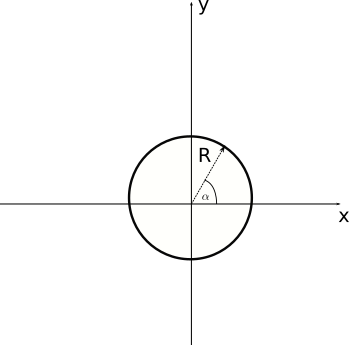
\includegraphics[height=5cm]{../images/6diszlokkor.png}
\caption{ Kör alakú diszlokációhurok.}
 \label{korabra}
 \end{center}
\end{figure}

Mekkora a diszlokációhurokra ható eredő forgatónyomaték nagysága? Válaszunkat $R$, $\sigma_0$ és $b$ segítségével adjuk meg!
\\

\textbf{Gy2.}  A koordináta-rendszerünk $x-y$ síkjában egy olyan  diszlokációhurok  fekszik, amelynek alakja $R$ sugarú kör (\ref{korabra2} ábra), Burgers-vektora (b,0,0). Az anyagot homogén megnyírjuk úgy, hogy  a feszültségtenzor nemzérus elemei $\sigma_{xy} = \sigma_{zx} = \sigma_0$.

Mekkora a diszlokációhurok egyik félkörére ható eredő erő nagysága?
Válaszunkat$R$, $\sigma_0$ és $b$ segítségével adjuk meg!
\begin{figure}[h!]
\begin{center}
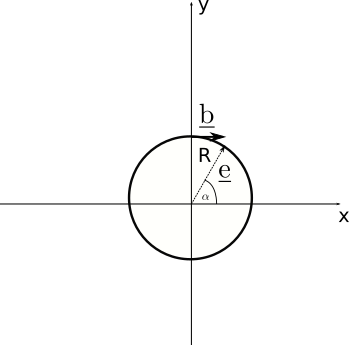
\includegraphics[height=7cm]{../images/6diszlokkor2.png}
\caption{ Kör alakú diszlokációhurok.}
 \label{korabra2}
 \end{center}
\end{figure}

Mekkora a diszlokációhurokra ható eredő forgatónyomaték nagysága? Válaszunkat $R$, $\sigma_0$ és $b$ segítségével adjuk meg!
\\

\textbf{Megoldás}

A Peach-Koehler formula alapján $\underline{F}=\underline{l}\times(\underline{\underline{\sigma}}\underline{b})$.

$$ \underline{\underline{\sigma}}\underline{b}= 
\begin{pmatrix} 0 & 0 & \sigma_0\\ 0 & 0 & 0 \\ \sigma_0 & 0 & 0 \end{pmatrix} \begin{pmatrix} b \\ 0\\ 0\end{pmatrix} = \begin{pmatrix} 0 \\ 0\\  \sigma_0 b \end{pmatrix}$$

Most írjuk fel a diszokáció irányvektorát, vagyis adott sugárhoz tartozó érintőt $\mathrm{d}\underline{l}$-t
$$ \underline{r} = R\begin{pmatrix} \cos \alpha \\ \sin \alpha \\  0 \end{pmatrix} \longrightarrow \mathrm{d}\underline{l} = R\begin{pmatrix} -\sin \alpha \\ \cos \alpha \\  0 \end{pmatrix}\mathrm{d}\alpha$$ 
Így adódik az adott hurokdarabra ható erő
$$\mathrm{d}\underline{F}=R\mathrm{d}\alpha \begin{pmatrix} -\sin \alpha \\ \cos \alpha \\  0 \end{pmatrix} \times \begin{pmatrix} 0 \\ 0\\  \sigma_0 b \end{pmatrix}=R \sigma_0 b \begin{pmatrix} \cos \alpha \\ \sin \alpha \\  0 \end{pmatrix}\mathrm{d}\alpha$$
Ebből a $+y$ félsíkon fekvő félkörre ható erőt integrálással kapjuk
$$\underline{F} = \int_{0}^{\pi} R \sigma_0 b \begin{pmatrix} \cos \alpha \\ \sin \alpha \\  0 \end{pmatrix}\mathrm{d}\alpha = 2 R \sigma_0 b \begin{pmatrix} 0 \\ 1 \\  0 \end{pmatrix}$$ 


\end{document}